\item We know that the solution to the $2-$D heat equation
$u_t = u_{xx} + u_{yy}$, with $u(x, y, 0) = f(x, y)$ is
%
\begin{align}
  u(x, y, t)
  & = \frac{1}{4 \pi t} \int^\infty_{-\infty} \int^\infty_{-\infty}
  f(\xi, \eta) e^{-\frac{(x - \xi)^2 + (y - \eta)^2}{4t}} \text d\xi \text d\eta
\end{align}

If
%
\begin{align}
  f(x, y) & =
  \begin{cases}
    1 & 2 \leq r \leq 4, r = \sqrt{x^2 + y^2}\\
    0 & \text{otherwise}
  \end{cases}
\end{align}

Sketch $u(x, y, t)$ for different $t$ values, say $t = 0, 5, 100, \infty$
\bigbreak
%_____________________________________________________________________________%

Note, as $t$ increases, the sharp edges near the top of the cylinder tend to smooth out. The drawings do not accurately represent this detail.

\begin{center}
  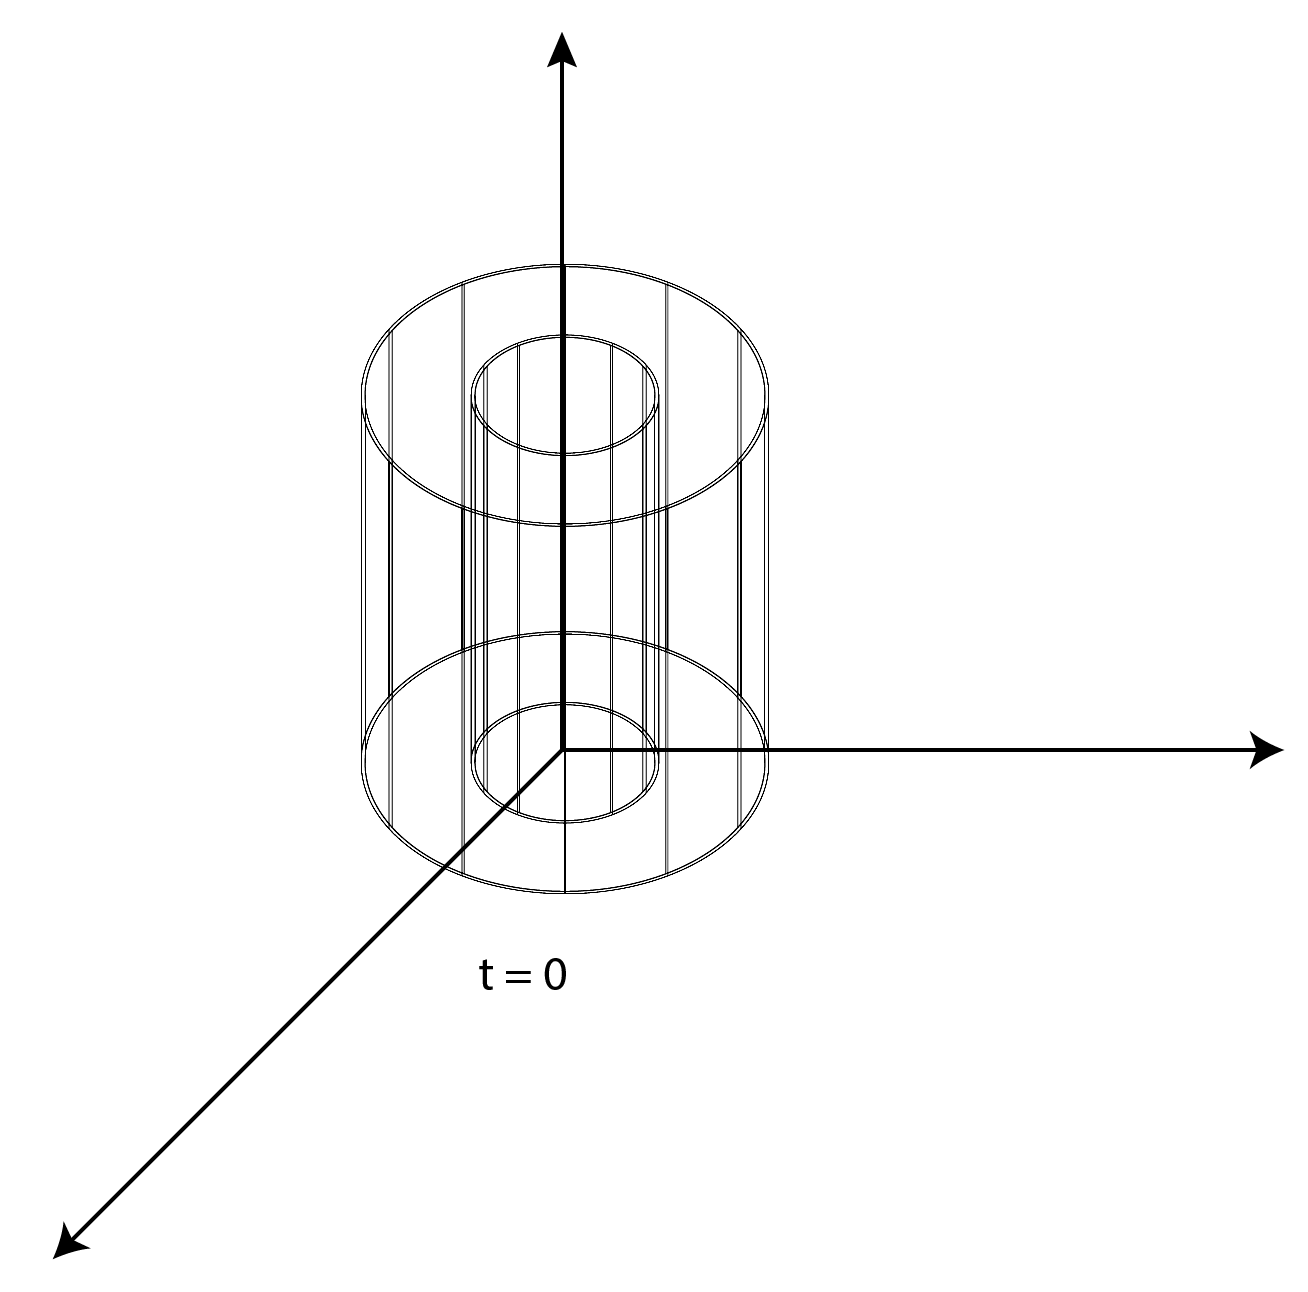
\includegraphics[height=8cm]{5-a}
  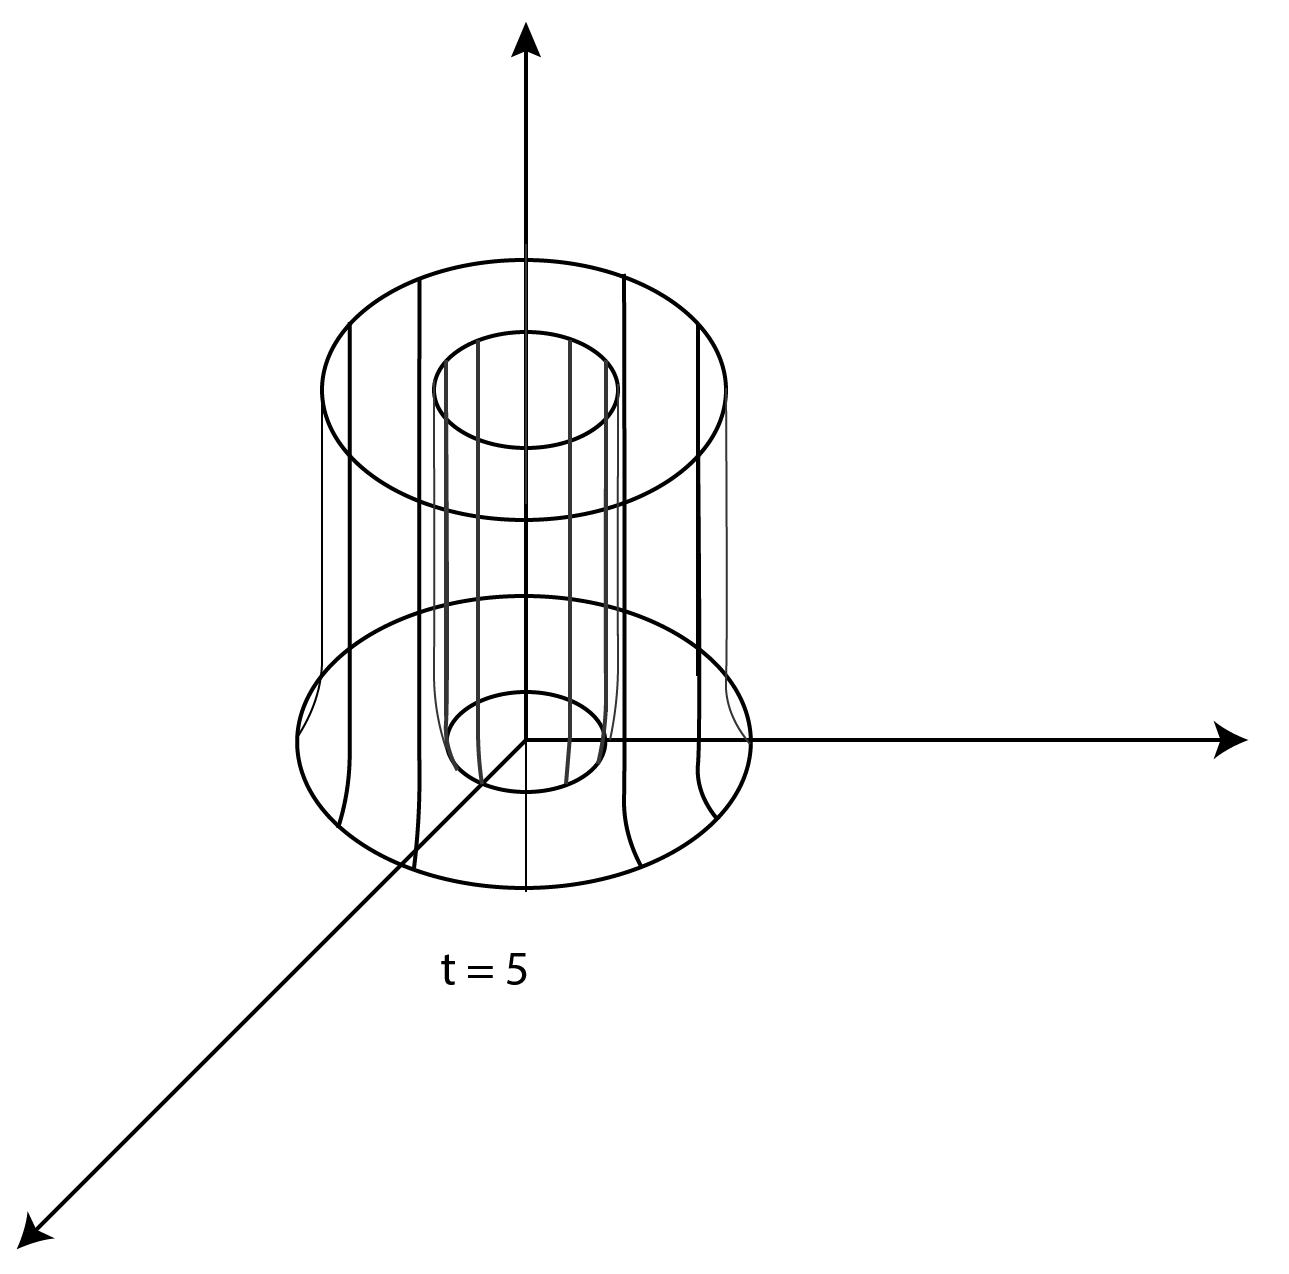
\includegraphics[height=8cm]{5-b}
  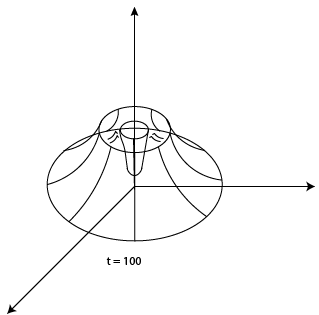
\includegraphics[height=8cm]{5-c}
  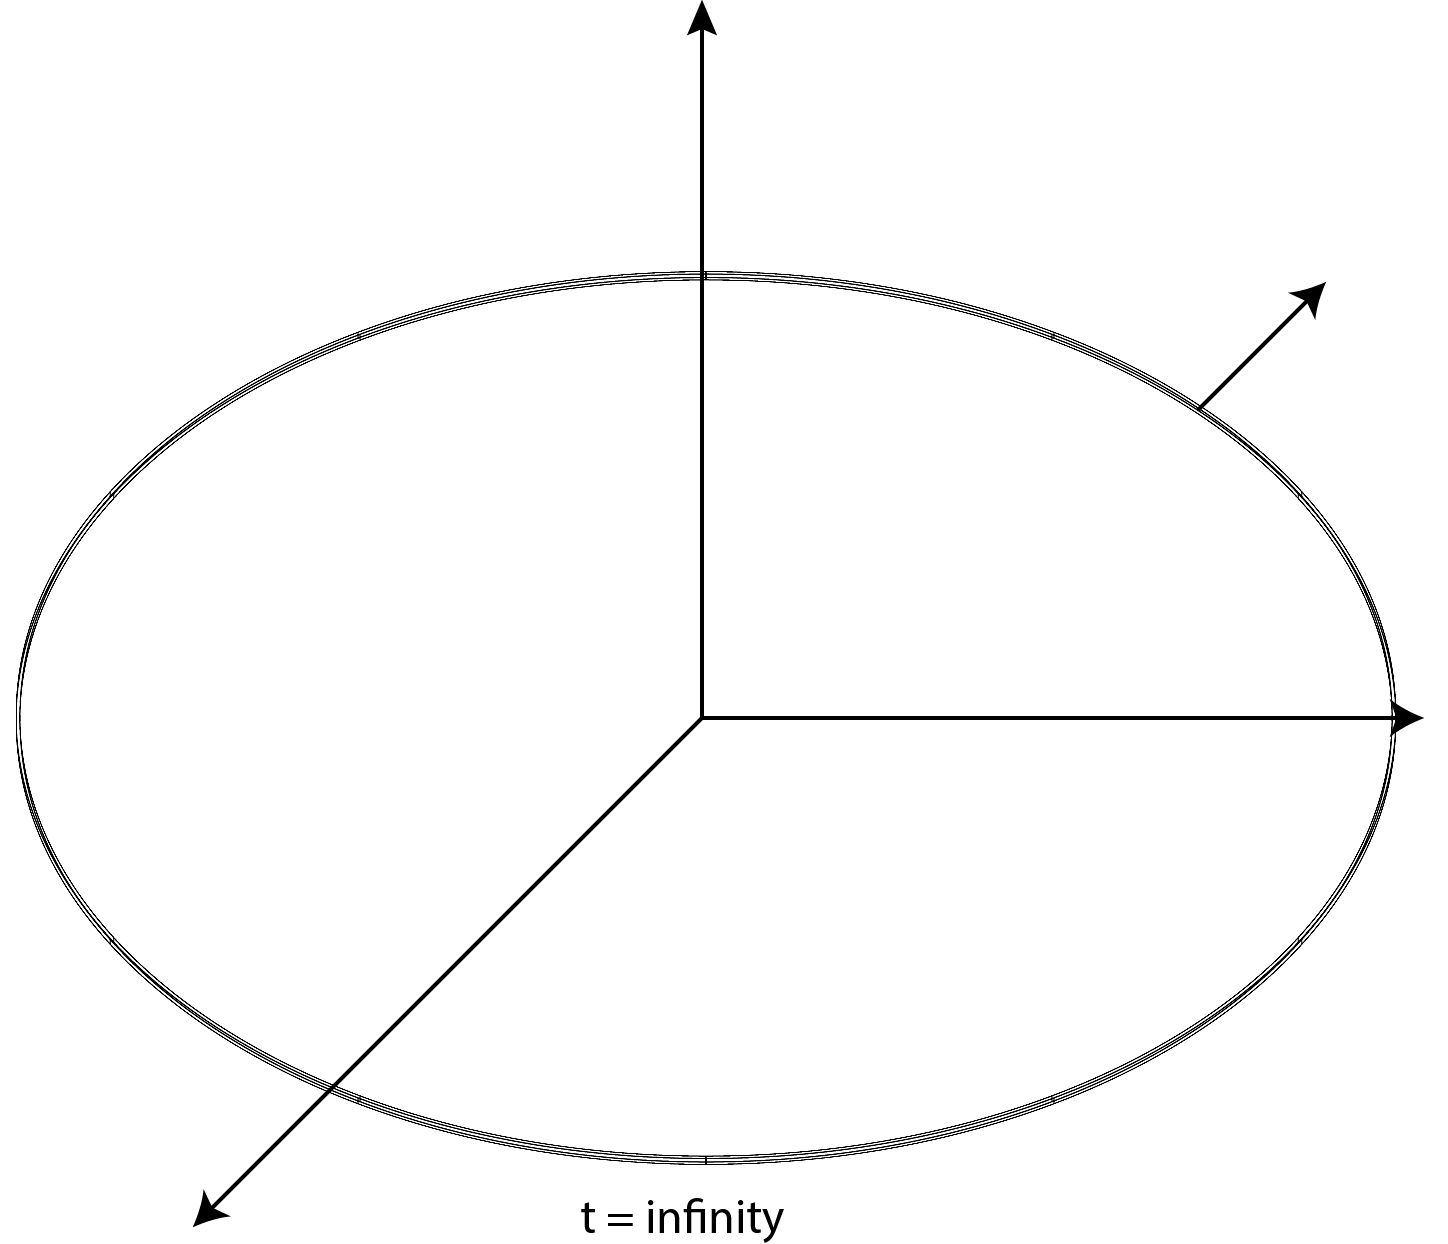
\includegraphics[height=8cm]{5-d}
\end{center}
